\section{CQ3}

\begin{fancyquote}
    \textbf{CQ3a)} How many separate observe notifications have been sent containing values for the resource ``/dining\_room/temperature'', ignoring retransmissions?\\
    \textbf{CQ3b)} How many of the notifications found in point CQ3a) are useless (e.g., a waste of traffic)?
\end{fancyquote}

\vspace{0.3cm}

\noindent
\begin{minipage}{\linewidth}
\subsection*{CQ3a - Identify the Token for \texttt{/dining\_room/temperature}}
Filter the URI path to \texttt{dining\_room/temperature}:
\begin{lstlisting}
tshark -r A.pcapng -Y "coap.code == 1 && coap.opt.observe == 0" -T fields -e coap.token -e coap.opt.uri_path | grep "dining_room,temperature" | awk '{print $1}' | sort -u
\end{lstlisting}
\vspace{-0.2cm}
\begin{figure}[H]
    \centering
    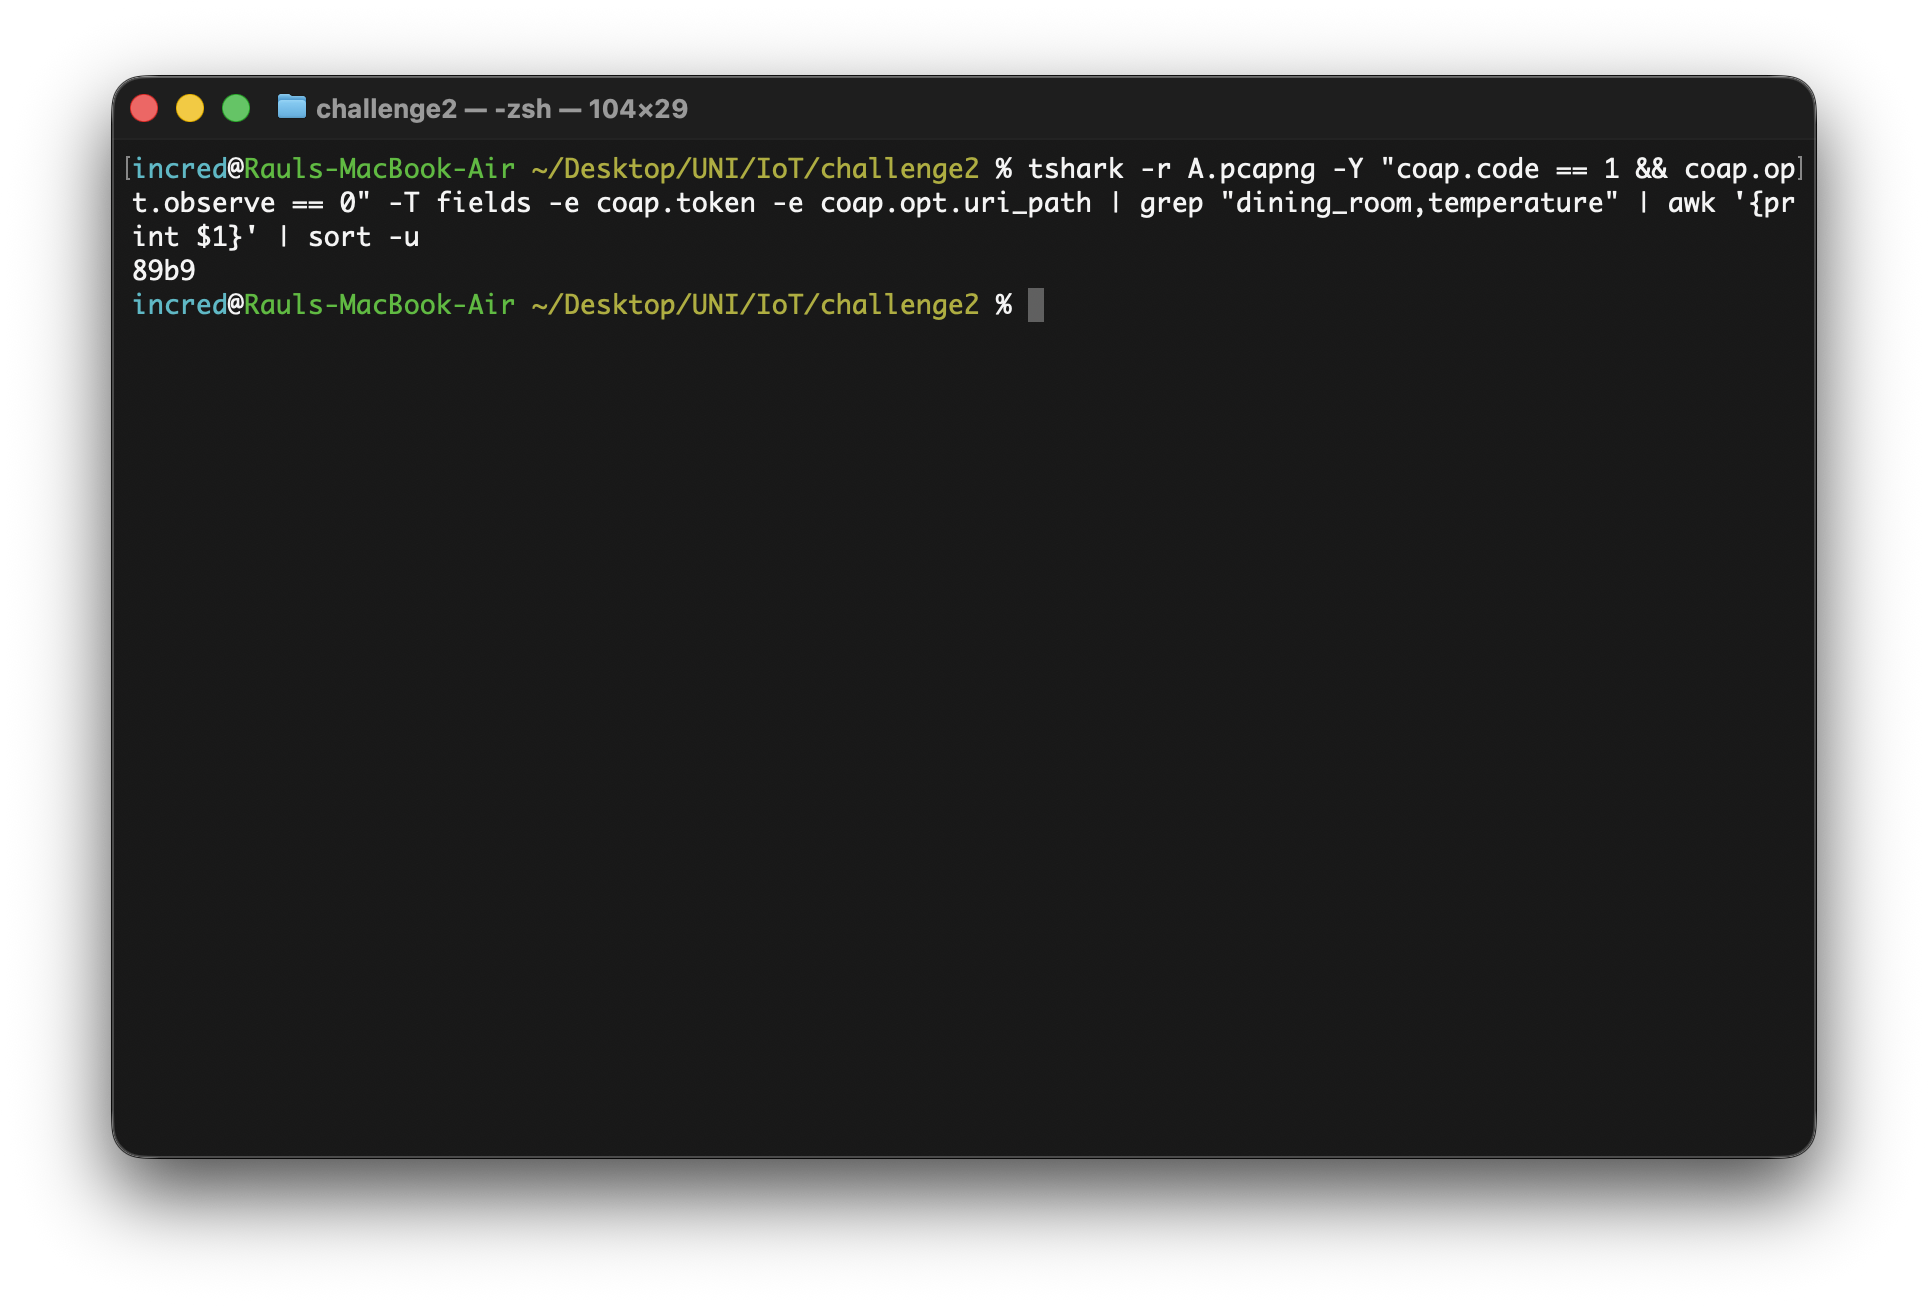
\includegraphics[width=0.75\linewidth]{images/cq3-token.png}
\end{figure}
\end{minipage}

\vspace{0.5cm}

\subsection*{CQ3a - Count Separate Observe Notifications}
Extract the notifications sent by the server. Notifications use the response code \texttt{2.05 Content} (Integer value: 69) and contain the \texttt{coap.opt.observe} field (which acts as a sequence number). To ignore retransmissions, we must filter out packets that have the same Observe sequence number. Retransmitted notifications carry the exact same sequence number as the original.

\vspace{0.2cm}

\noindent
\begin{minipage}{\linewidth}
\subsubsection*{Extract all notifications for the token}
\begin{lstlisting}
tshark -r A.pcapng -Y "coap.code == 69 && coap.opt.observe" -T fields -e coap.token -e coap.opt.observe -e coap.payload | grep -f CQ3/obs_token.txt > CQ3/all_notifications.txt
\end{lstlisting}
Extracts the Token, Observe Sequence Number, and Payload for all notifications, filtering strictly for the Token.
\vspace{0.1cm}
\begin{figure}[H]
    \centering
    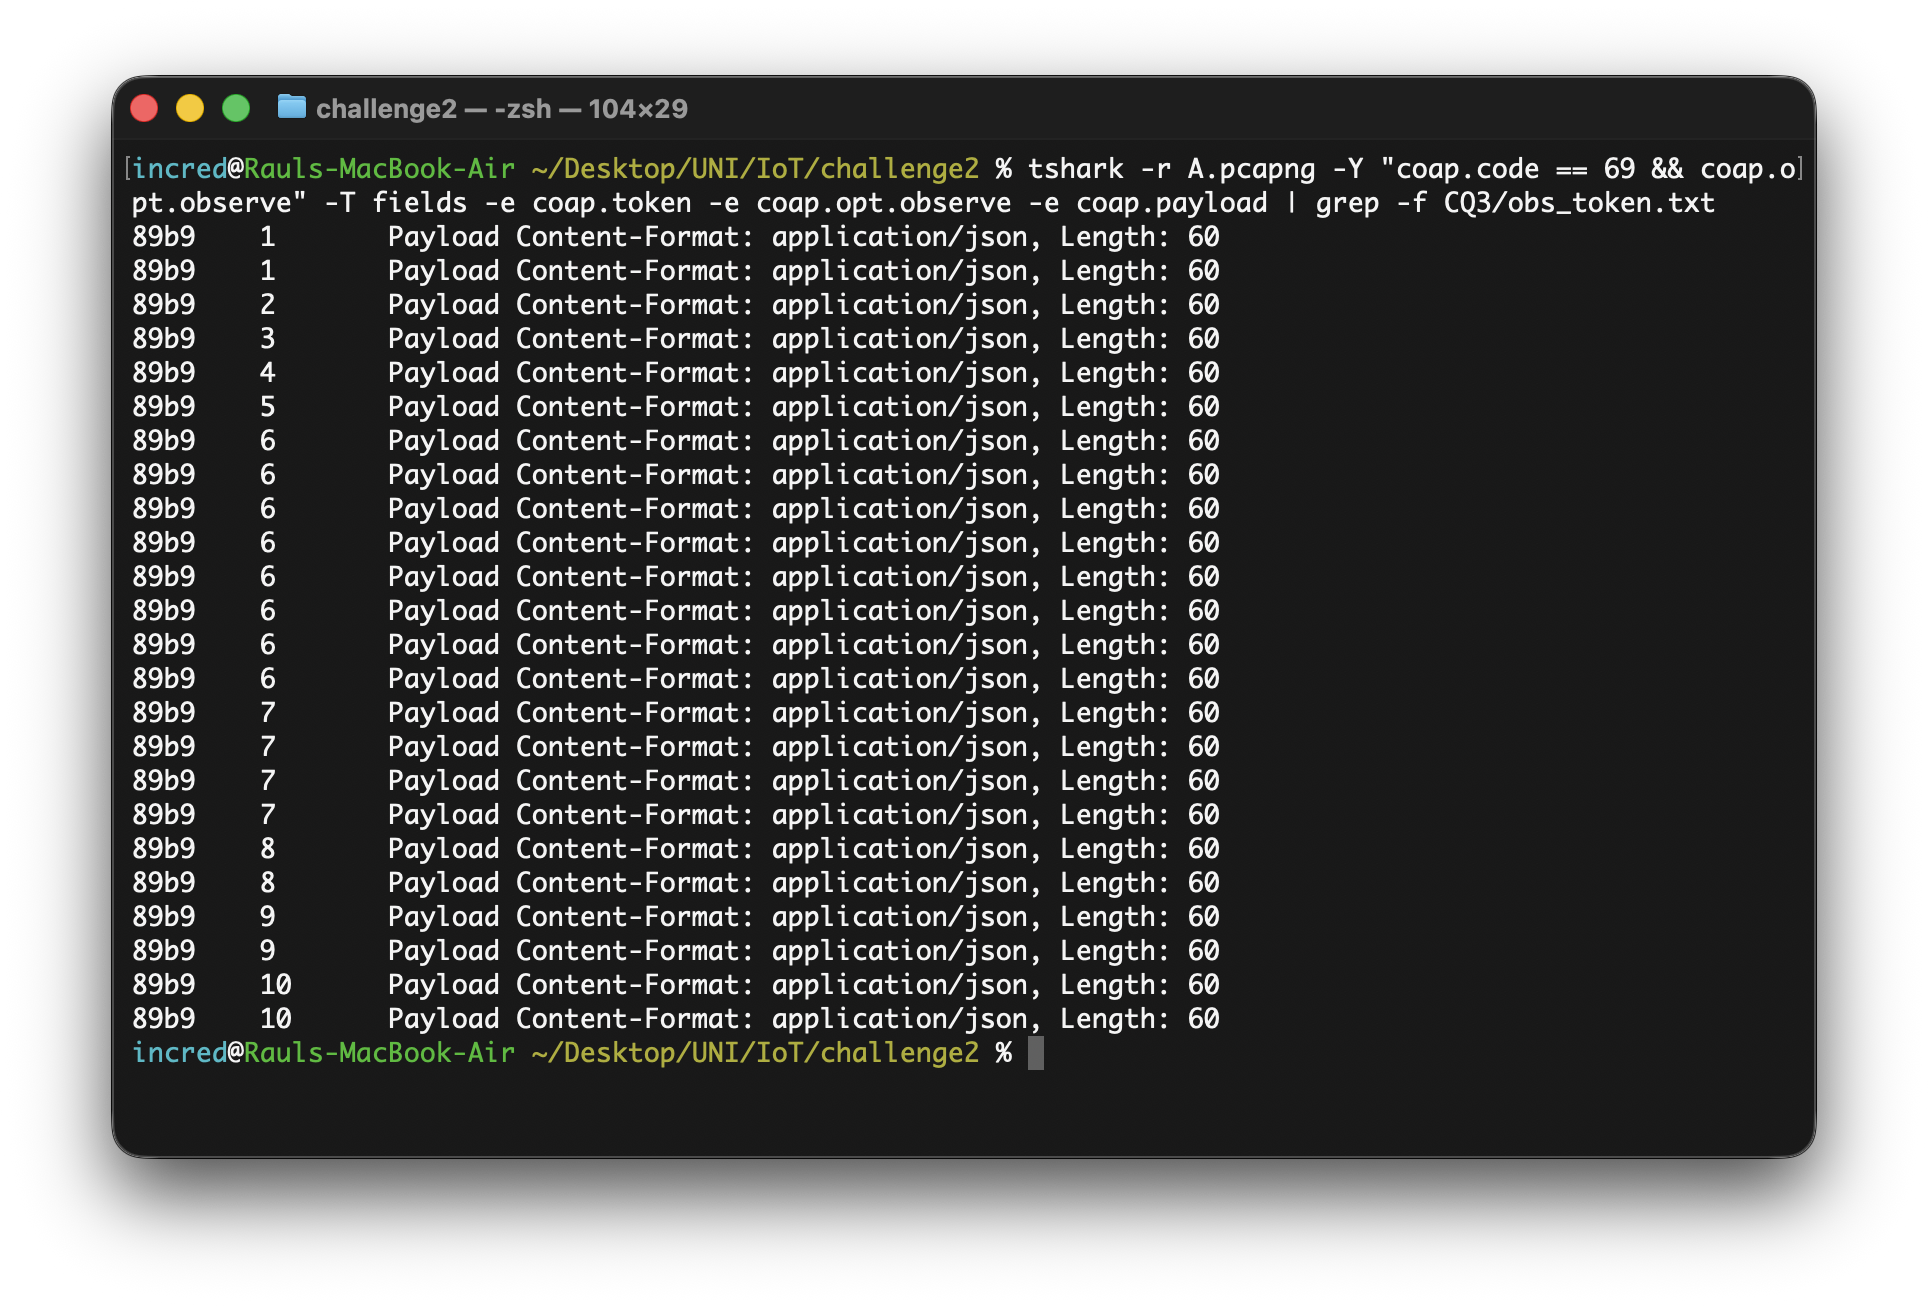
\includegraphics[width=0.75\linewidth]{images/cq3-notifications.png}
\end{figure}
\end{minipage}

\vspace{0.5cm}

\noindent
\begin{minipage}{\linewidth}
\subsubsection*{Filter retransmissions and count}
\begin{lstlisting}
sort -u -k2,2n CQ3/all_notifications.txt > CQ3/unique_notifications.txt
wc -l < CQ3/unique_notifications.txt
\end{lstlisting}
\textbf{\texttt{sort -u -k2,2n}}: Sorts the file numerically (\texttt{n}) based purely on the second column (\texttt{-k2,2}), which is the Observe Sequence Number. The \texttt{-u} flag ensures that if multiple packets have the exact same sequence number (retransmissions), only the first one is kept.
\vspace{0.1cm}
\begin{figure}[H]
    \centering
    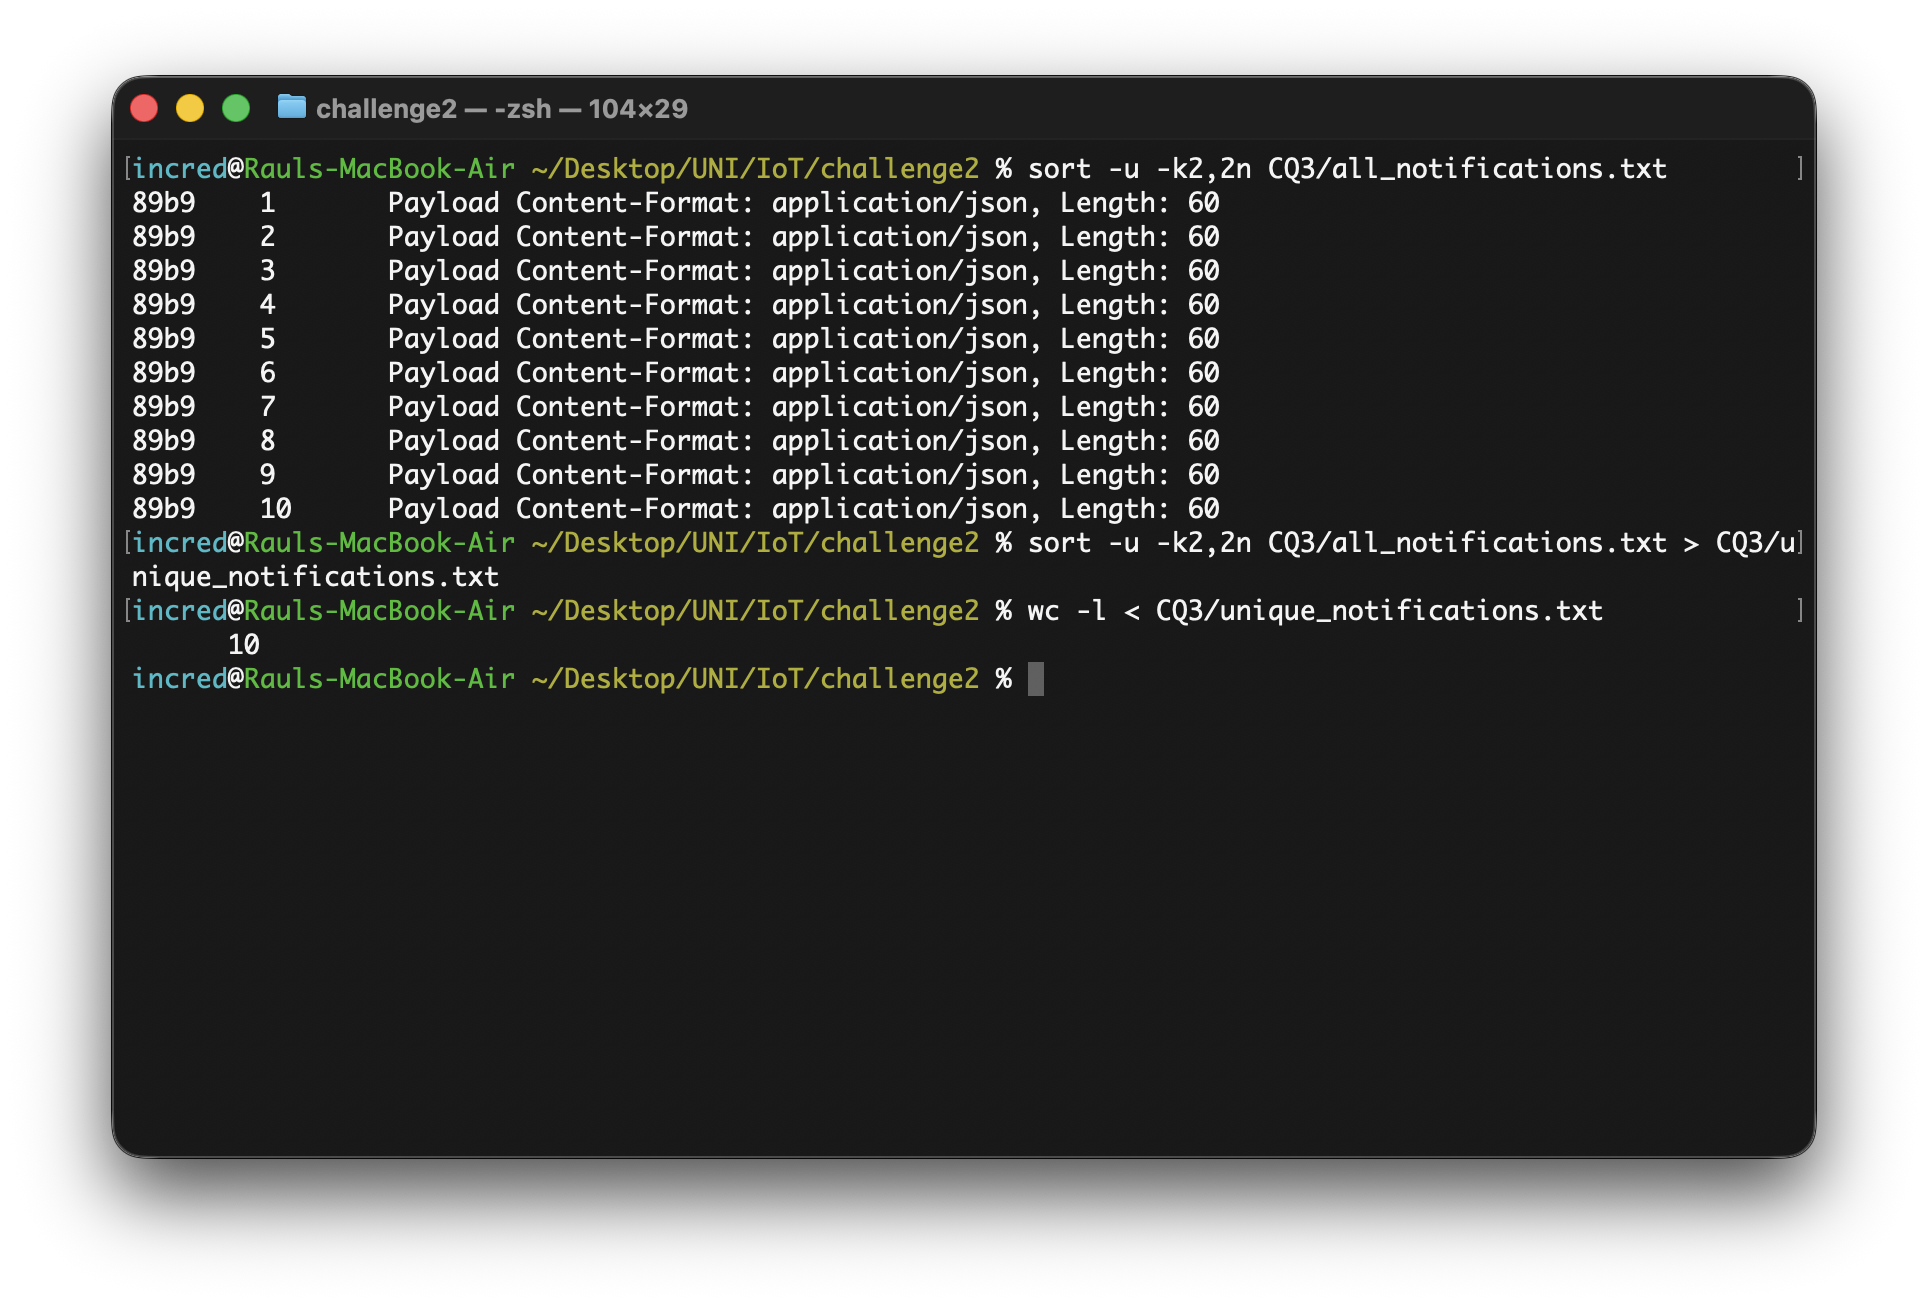
\includegraphics[width=0.75\linewidth]{images/cq3a-result.png}
\end{figure}

\vspace{0.2cm}
\textbf{\huge Answer CQ3a: 10}
\end{minipage}

\noindent
\begin{minipage}{\linewidth}
\subsection*{CQ3b - How many notifications are useless?}

For CQ3b, only the notifications already identified in CQ3a must be considered, therefore retransmissions remain excluded.  
Based on the clarification given for the assignment, a notification should be considered mainly useless if it is sent but not effectively received/processed.

First, I listed the 10 unique notifications found in CQ3a together with their CoAP type, MID, and Observe sequence number:

\begin{lstlisting}
tshark -r A.pcapng -Y "coap.token == 89b9 && coap.code == 69 && coap.opt.observe" -T fields -e frame.number -e coap.type -e coap.mid -e coap.opt.observe | sort -u -k4,4n
\end{lstlisting}

This produced:

\begin{verbatim}
4344  2  10588  1
5098  0  38     2
5623  0  43     3
8509  0  45     4
9414  0  49     5
9866  0  54     6
10573 0  62     7
11220 0  74     8
11917 0  87     9
12782 0  90     10
\end{verbatim}

The first notification is already an ACK-type message (\texttt{coap.type == 2}), while the others are Confirmable notifications (\texttt{coap.type == 0}).  
For each Confirmable notification, I checked whether a corresponding ACK with the same MID exists:

\begin{lstlisting}
tshark -r A.pcapng -Y "coap.type == 2 && (coap.mid == 38 || coap.mid == 43 || coap.mid == 45 || coap.mid == 49 || coap.mid == 54 || coap.mid == 62 || coap.mid == 74 || coap.mid == 87 || coap.mid == 90)" -T fields -e frame.number -e coap.mid
\end{lstlisting}

The result was:

\begin{verbatim}
5099  38
5629  43
8510  45
9415  49
\end{verbatim}

Therefore, ACKs were found only for MIDs \texttt{38}, \texttt{43}, \texttt{45}, and \texttt{49}.  
No ACK was found for MIDs:

\begin{verbatim}
54, 62, 74, 87, 90
\end{verbatim}

These 5 notifications were sent but do not appear to have been successfully confirmed, so they are considered useless according to the intended interpretation of the question.

\vspace{0.4cm}
\textbf{\huge Answer CQ3b: 5}
\end{minipage}